\subsection{Configurable Agentic Runtime}
\label{sec:method_runtime}

\subsubsection{YAML Configuration Schema}

The runtime follows a configuration-as-code model in which each agent variant is represented by a single YAML file. This file specifies the reasoning model, embedding model, system prompt, optional planning prompt, per-tool query-analyzer prompts, tool exposure, and flow strategy. The design choice is deliberate: researchers should be able to version-control an agent definition, rerun it on a new tenant, and attribute behavioral changes to the configuration diff rather than to hidden code edits.

\begin{figure}[t]
\centering
\begin{minipage}{0.92\linewidth}
\begin{lstlisting}[basicstyle=\color{blue}\small\ttfamily]
id: react-agent-v1
version: "1.0.0"
model:
  provider: azure
  name: gpt-4o
  parameters: {temperature: 0.7}
embedding:
  provider: azure
  model: text-embedding-ada-002
system_prompt: |
  You are an intelligent enterprise assistant.
  {user_profile}
query_analyzer_prompt:
  search_email: |
    Analyze the user's email query and return
    strategy, refined_query, and sender_name.
tools:
  definitions:
    - search_email
    - search_file
    - search_meeting
    - search_people
    - read_file
    - execute_python
flow:
  strategy: react
  max_turns: 5
\end{lstlisting}
\end{minipage}
\caption{Condensed runtime configuration illustrating how model choice, prompt behavior, tool exposure, and flow strategy are all declared in YAML.}
\label{lst:runtime_yaml}
\end{figure}

\begin{table}[h]
\centering
\caption{Six runtime dimensions that can be changed without source-code edits.}
\label{tab:runtime_dimensions}
\small
\begin{tabular}{p{0.17\linewidth}p{0.24\linewidth}p{0.48\linewidth}}
\toprule
\textbf{Dimension} & \textbf{Configuration field} & \textbf{Research question enabled} \\
\midrule
Reasoning model & \texttt{model.*} & How sensitive is performance to the underlying LLM family and decoding parameters? \\
Embedding model & \texttt{embedding.*} & How much of end-to-end performance is driven by retrieval quality rather than reasoning quality? \\
Cognitive architecture & \texttt{flow.strategy} & Does ReAct or plan-and-execute better handle multi-step enterprise tasks? \\
Global prompting & \texttt{system\_prompt}, \texttt{planning\_prompt} & How do role instructions and planning structure affect behavior and citation quality? \\
Tool exposure & \texttt{tools.definitions} & Which tools are necessary for each query type, and what are the failure modes when they are removed? \\
Sandbox implementation & tool dependencies and runtime backend & How do local, remote, or more restrictive execution environments change tool use? \\
\bottomrule
\end{tabular}

\end{table}

\subsubsection{Cognitive Architectures}

EABench currently exposes two cognitive architectures. Under the \texttt{react} strategy, the runtime loops through thought, tool call, observation, and response generation until the model emits a final answer or reaches a hard turn limit. Under the \texttt{researcher} strategy, the runtime first invokes a planner to produce a structured plan and then executes that plan with the normal tool-enabled loop. The second strategy adds overhead, but it is often better suited to multi-hop cases in which the agent must identify a dependency chain before any single tool call is obviously useful.

\begin{table}[t]
\centering
\caption{Comparison of the two built-in runtime strategies.}
\label{tab:strategy_compare}
\small
\begin{tabular}{p{0.16\linewidth}p{0.18\linewidth}p{0.18\linewidth}p{0.30\linewidth}}
\toprule
\textbf{Strategy} & \textbf{First action} & \textbf{Typical strength} & \textbf{Typical failure mode} \\
\midrule
ReAct & Immediate tool-enabled reasoning & Fast response on local retrieval tasks & Can drift on long dependency chains or overlook needed decomposition \\
Researcher & Tool-free planning pass & Stronger structure on multi-step tasks & Higher token usage and possible over-planning on simple cases \\
\bottomrule
\end{tabular}

\end{table}

\begin{figure}[t]
\centering
%\fbox{\parbox{0.96\linewidth}{%
%\vspace{4pt}
%\small\color{blue}\itshape\raggedright
%\textbf{[Figure placeholder --- generation pending.]}
%A side-by-side two-panel comparison diagram separated by a vertical dashed center line, with a shared header banner.
%\textbf{Header banner (spanning both panels):} A YAML code snippet showing \texttt{flow.strategy: react} (left half) and \texttt{flow.strategy: researcher} (right half), with bold label above: ``EABench-configurable strategy selection (single YAML field).''
%\textbf{Left panel --- ReAct:}
%Vertical stack of rounded boxes connected by solid downward arrows:
%(1)~``User Query'' box (deep blue, top);
%(2)~``Reasoning'' box (amber) annotated with a thought-bubble: ``Which tool is needed and why?'';
%(3)~``Action'' box (orange) showing a tool-call icon with parameter fields;
%(4)~``Observation'' box (teal) showing a tool-result snippet.
%A curved dashed arrow on the left side of the stack loops from the Observation box back up to the Reasoning box, labeled ``repeat until answer ready.''
%A final ``Answer'' box (green) sits below Observation after the loop terminates, connected by a solid arrow.
%\textbf{Right panel --- Plan-and-Execute:}
%Two vertically stacked phases with a horizontal divider:
%\textit{Phase~1 ``Plan''}: A ``Planner LLM'' box (deep blue) outputs a numbered clipboard: Step~1, Step~2, \ldots, Step~N.
%A thick downward arrow labeled ``hand off complete plan'' leads to:
%\textit{Phase~2 ``Execute''}: An ``Executor'' rounded rectangle (orange) that loops through each step, showing \textit{(Step $i$)} $\rightarrow$ Tool Call (orange) $\rightarrow$ Observation (teal) for each step, with a small inner circular arrow labeled ``steps~1\ldots N.''
%A ``Final Answer'' box (green) sits below the executor after all steps complete.
%\textbf{Annotation differences:} The ReAct panel is narrower and denser; the Plan-and-Execute panel is taller with a clear two-phase separation.
%Color scheme: query/answer boxes in deep blue and green; reasoning/planning in amber; action/execution in orange; observations in teal; dashed loop arrows in gray.
%\vspace{4pt}
%}}
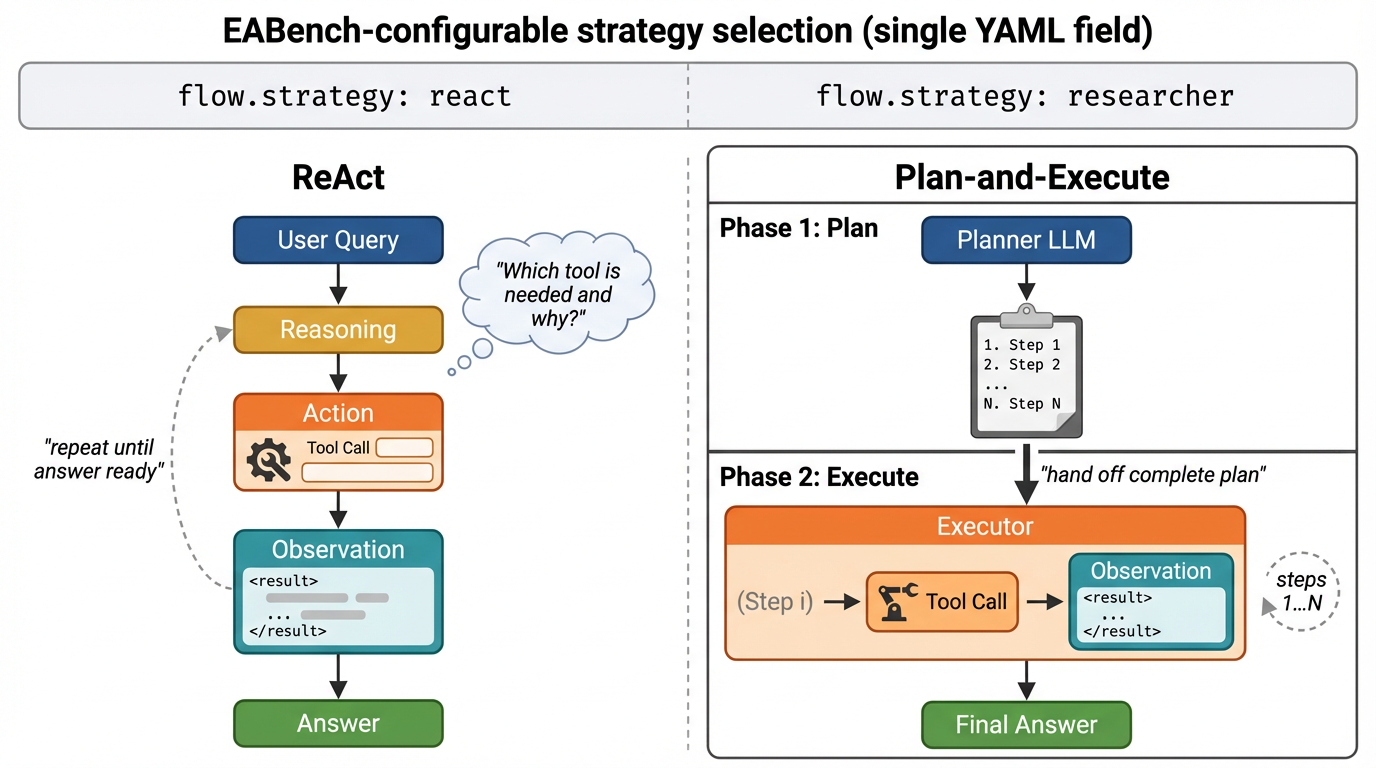
\includegraphics[width=0.9\textwidth]{figures/agent-architecture-config.png}
\caption{The two cognitive architectures natively supported by EABench as hot-swappable \texttt{flow.strategy} values. ReAct (left) interleaves reasoning and acting in a tight feedback loop; Plan-and-Execute (right) separates a global planning phase from sequential step-wise execution, reducing context drift on long multi-hop tasks.}
\label{fig:cognitive_arch}
\end{figure}

\subsubsection{Multi-Provider LLM Support}

The runtime separates the configuration schema from the provider implementation through a common LLM interface. Provider choice is driven by the YAML field \texttt{model.provider}, while credentials and deployment-specific settings are resolved from environment variables. This separation makes provider swapping operationally cheap: researchers can move between OpenAI, Azure-hosted deployments, or compatible local endpoints while preserving the rest of the runtime definition. That property is especially important for cross-model evaluations, because it prevents provider migration from becoming a hidden code change.

\subsubsection{Enterprise Tool Suite and Search Infrastructure}

The built-in tool suite combines semantic retrieval tools with sandboxed execution tools. Search tools cover emails, files, meetings, people, one-to-one chats, group chats, and channel messages. Execution tools cover file inspection, directory listing, shell execution, and Python execution. Tools are registered through a decorator-based registry that automatically exports JSON schemas for model-facing tool calling, while dependencies such as the sandbox, search engine, and query analyzer are injected by the runner. This keeps tool implementations modular and makes tool ablations straightforward: removing a tool from the YAML file is sufficient to change the agent's action space.

Retrieval itself is implemented as a set of separate vector indices rather than as one monolithic store. EABench indexes at least nine content collections, including file snippets, full file contents, emails, chats, group chats, channels, meeting metadata, meeting transcripts, and user profiles. Similarity is computed with cosine similarity, and the resulting embeddings are cached on disk to avoid recomputation across repeated evaluations. The indices are filtered by user context before results are returned, which means the runtime and the evaluator both observe the same access-controlled search space.

\subsubsection{Query Analyzer}

An optional LLM-driven query analyzer sits between the user request and the retrieval tools. Instead of forwarding raw language directly to the vector index, the analyzer can refine a query, select a search strategy, or resolve a sender filter before retrieval occurs. Because its prompts are themselves configurable in YAML, EABench treats search refinement as a first-class experimental variable. Researchers can therefore study not only whether a search tool is useful, but whether specific decomposition heuristics or query rewrites materially improve retrieval fidelity.